\documentclass{article}
\usepackage[utf8]{inputenc}
\usepackage[spanish]{babel}
\usepackage{subcaption}
\usepackage{graphicx}
\graphicspath{ {images/} }

\usepackage{listings}
\lstdefinestyle{code}{
language=Octave,
frame=single,
breakatwhitespace=true,
breaklines=true,
basicstyle=\small\ttfamily,
tabsize=4,
numbers=left,
numberstyle=\tiny,
columns=fullflexible
}
\lstdefinestyle{snippet}{
language=Octave,
breakatwhitespace=true,
breaklines=true,
basicstyle=\small\ttfamily,
}

\addtolength{\textwidth}{1cm}

\title{Práctica 1}
\author{Héctor Laria Mantecón y Samuel Lapuente Jiménez}
\date{29 de octubre de 2015}

\begin{document}

\maketitle
\section{Introducción}
Dados unos ejemplos de entrenamiento, mediante varios métodos de regresión lineal llegamos a una función que estima el valor aproximado que deberían tomar las soluciones conforme a unas entradas cualesquiera.

\section{Regresión lineal con una variable}
Utilizamos el método de descenso de gradiente para minimizar la función de coste $J(\theta)$ que utiliza una hipótesis $h(\theta)$, dadas ambas en el enunciado. Para ello utilizamos los diferentes scripts que se detallan en las siguientes subsecciones.

Uniendo estos scripts tenemos:
\lstinputlisting[style=code]{src/uno.m}
\pagebreak

\subsection{gradientDesc.m}
Esta función realiza el descenso de gradiente para encontrar la recta que mejor se ajusta a los ejemplos de entrenamiento.
\lstinputlisting[style=code]{src/gradientDesc.m}
\pagebreak

\subsection{plotting.m}
Esta función imprime las gráficas \ref{fig:recta}, \ref{fig:coste} y \ref{fig:contorno}.
\lstinputlisting[style=code]{src/plotting.m}

\subsection{cost.m}
Esta función calcula el coste, implementando las fórmulas $J(\theta)$ y $h(\theta)$.
\lstinputlisting[style=code]{src/cost.m}

\begin{figure}
\begin{subfigure}{0.5\textwidth}
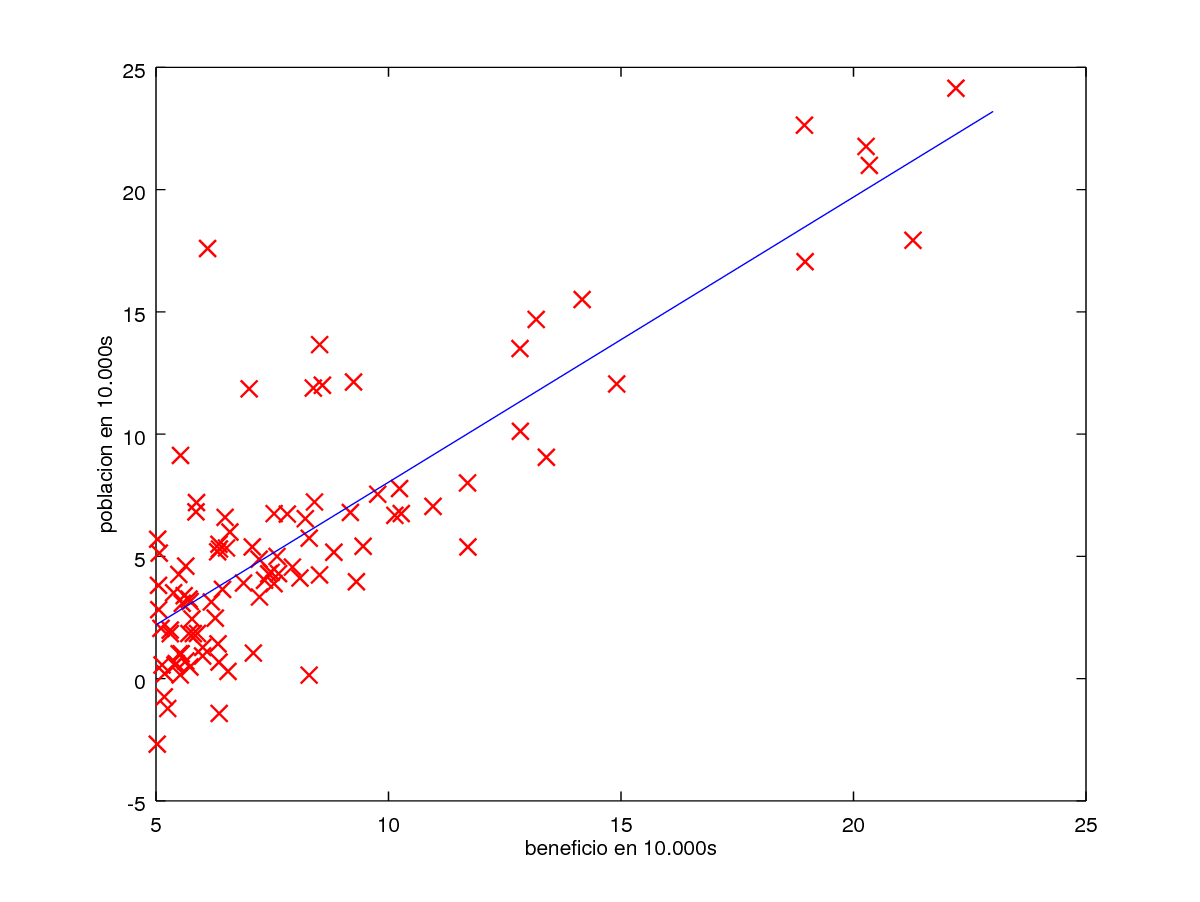
\includegraphics[width=\linewidth]{rectaRegresion}
\caption{}
\label{fig:recta}
\end{subfigure}
\begin{subfigure}{0.5\textwidth}
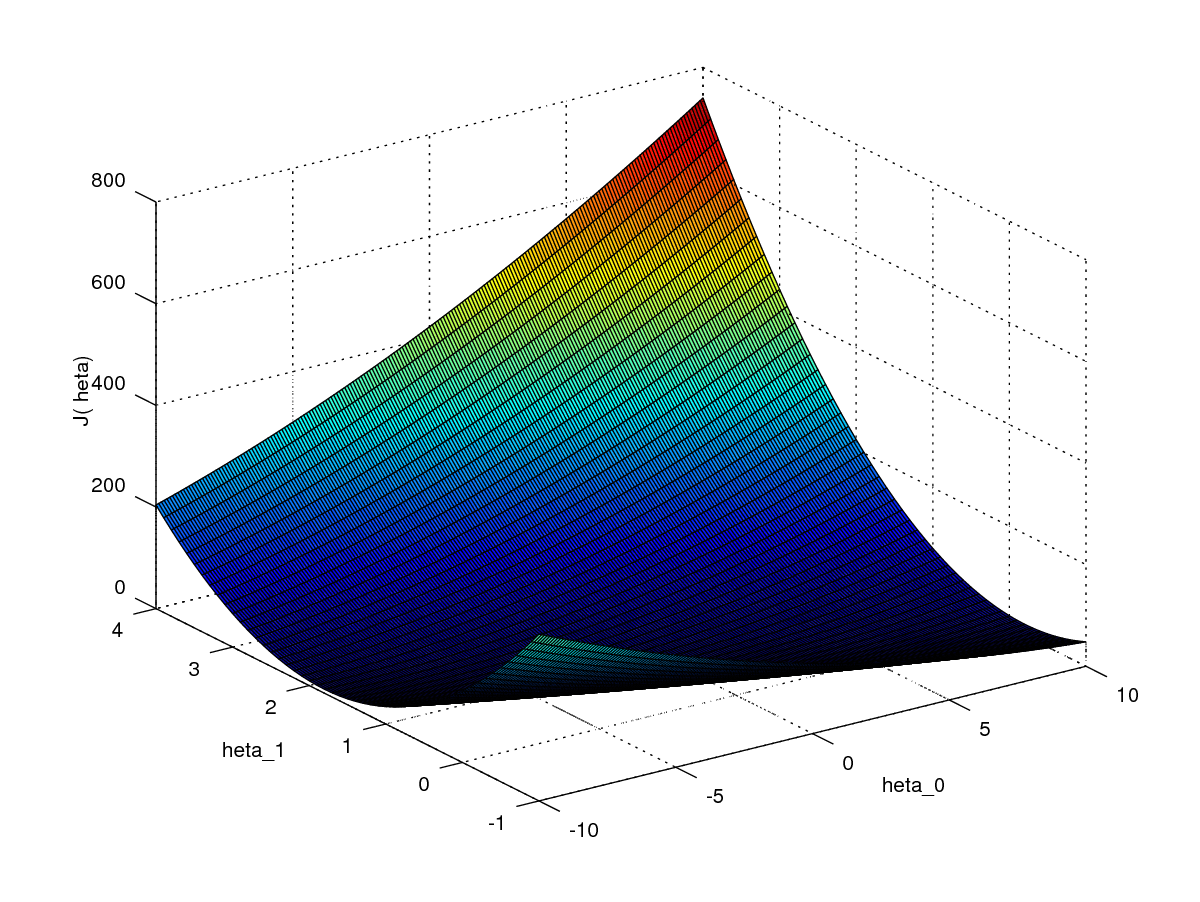
\includegraphics[width=\linewidth]{surfaceCoste}
\caption{}
\label{fig:coste}
\end{subfigure}

\begin{subfigure}{\textwidth}
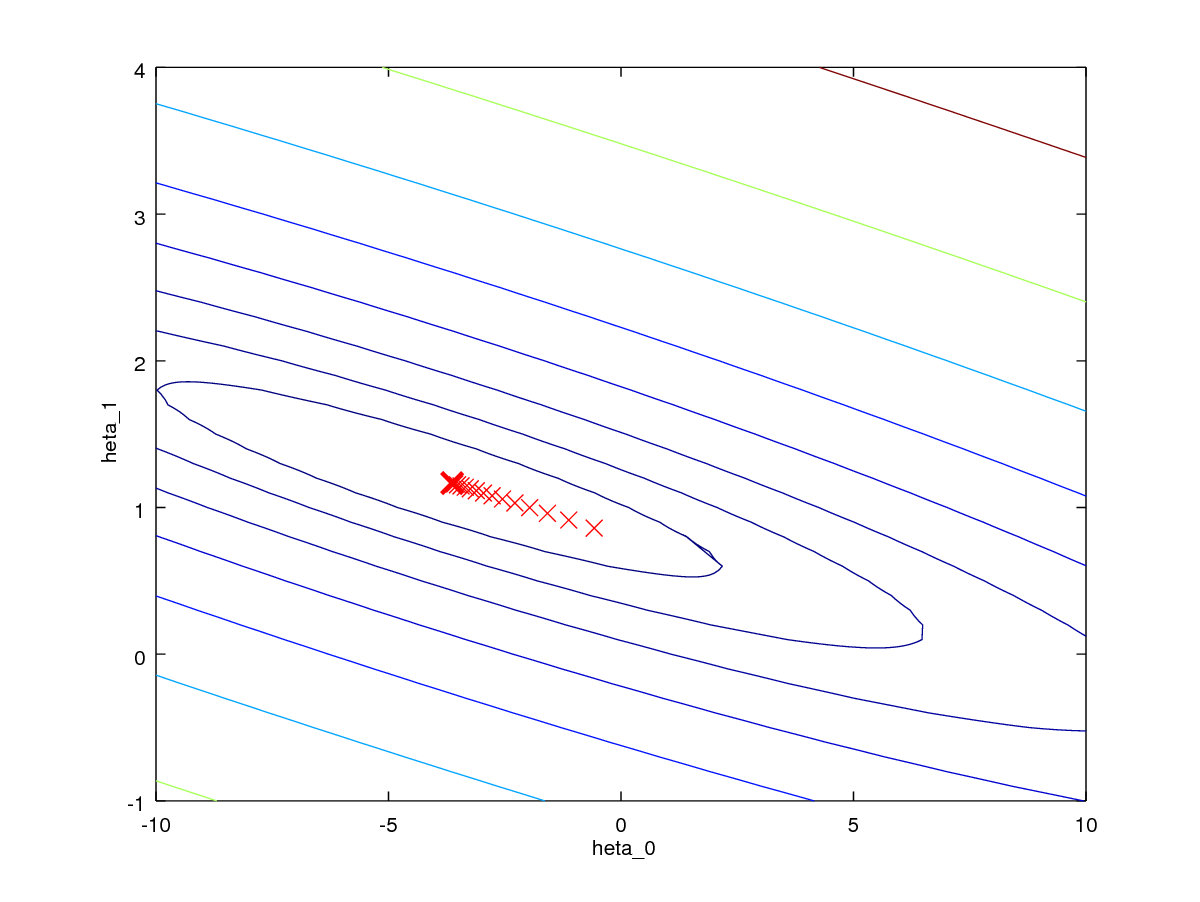
\includegraphics[width=\linewidth]{contourTheta}
\caption{}
\label{fig:contorno}
\end{subfigure}

\caption{Gráficas del primer apartado}
\end{figure}

\section{Regresión lineal con varias variables}
Ahora tenemos que aplicar el mismo método de regresión, teniendo varios atributos en los ejemplos de entrenamiento. El script principal es el siguiente:
\lstinputlisting[style=code]{src/dos.m}

\subsection{featureNormalize.m}
Lo primero que se pide es una función con esta cabecera:
\begin{lstlisting}[style=snippet]
function[X_norm, mu, sigma] = normalizaAtributo(X)
\end{lstlisting}
La cual es nuestra {\tt featureNormalize}.
\lstinputlisting[style=code]{src/featureNormalize.m}

\subsection{costMulti.m}
Hemos implementado la función $J$ como nos pedía en el cuadernillo.
\lstinputlisting[style=code]{src/costMulti.m}

\subsection{estudioMulti.m}
Y finalmente dibujamos las gráficas que nos piden, donde se muestra la evolución de la función de coste $J(\theta)$ a medida que avanza el descenso de gradiente, con distintos valores de tasa de aprendizaje.
\lstinputlisting[style=code]{src/estudioMulti.m}

\begin{figure}[h]
\centering
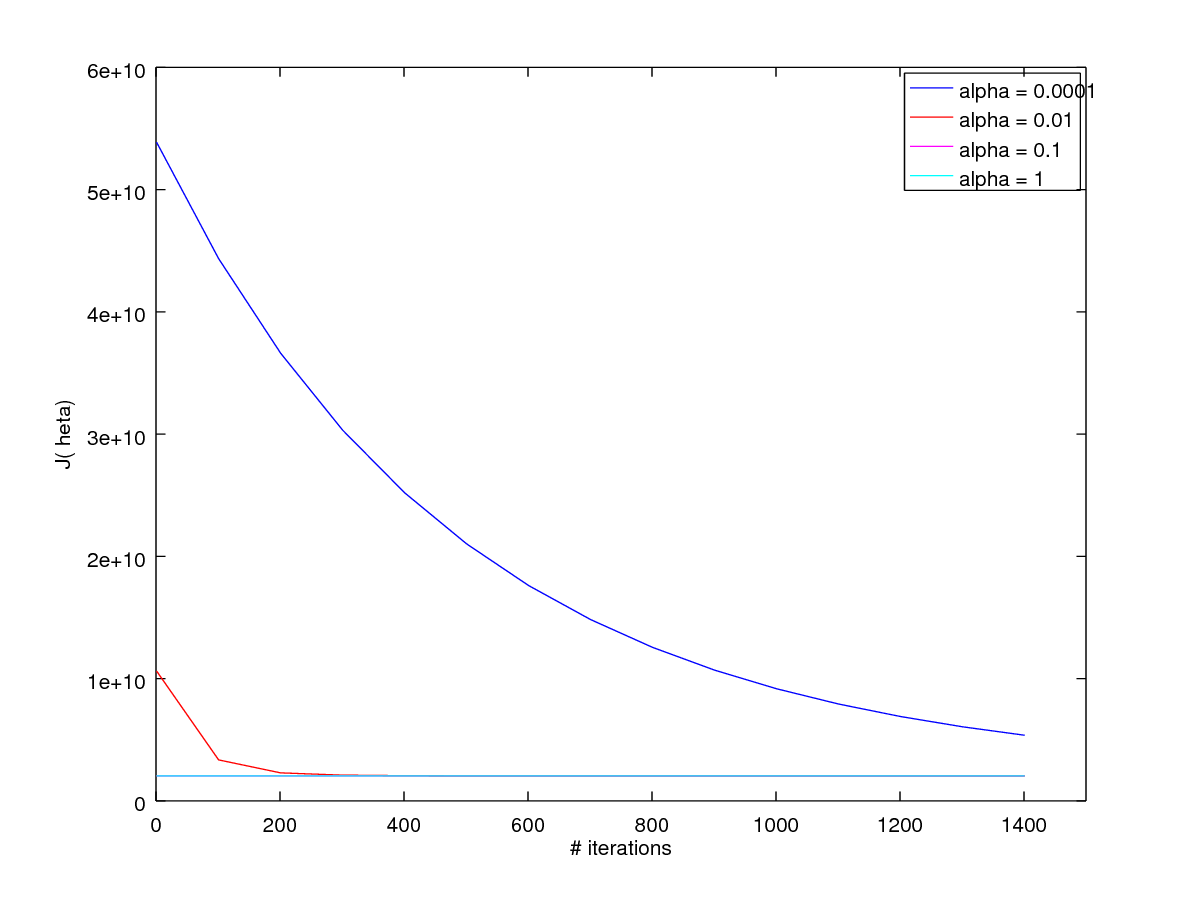
\includegraphics[width=\textwidth]{estudioMulti}
\label{fig:estudio}

\caption{Gráfica del segundo apartado}
\end{figure}
\pagebreak

\section{Conclusión}
Como podemos ver, el descenso de gradiente funciona correctamente ya que como se aprecia en la gráfica \ref{fig:recta}, la recta abarca el mayor número de puntos posibles ya que minimiza apropiadamente el coste de la gráfica \ref{fig:coste} como se ve en las sucesivas iteraciones del algoritmo, representado en la gráfica \ref{fig:contorno}.
\vspace{3mm}

Para la segunda parte hemos visto que la normalización ha reducido considerablemente el tiempo de cómputo de la regresión.
La salida del script principal es:
\begin{lstlisting}[style=snippet]
resultadoGradiente = 293100
resultadoNormal = 283360
\end{lstlisting}
pero es peor que una solución analítica (dada por la ecuación normal {\tt pinv(X' * X) * X' * y}) porque el descenso de gradiente no deja de ser una aproximación.

Interpretando la gráfica del segundo apartado, que muestra el descenso de gradiente con diferentes $\alpha$, vemos que con uno mayor se acerca mucho más rápido al óptimo pero corremos el riesgo de {\it saltárnoslo} y nunca llegar a él, por eso debemos valorar entre coger un $\alpha$ suficientemente grande o pequeño.


\end{document}
